% vim:ts=4:sw=4
% Copyright (c) 2014 Casper Ti. Vector
% Public domain.

\chapter{原型系统的设计与实现}
	\section{系统功能}
		系统主要有如下功能:

		1)社群划分。根据输入的时间信息,结合数据库中的高速公路收费信息,进行社群划分。

		2)关键路段挖掘。根据输入的时间信息,结合数据库中的高速公路收费信息,进行关键路段挖掘。

		3)静态挖掘。根据历史信息,稳定挖掘关键路段,给管理者提供参考。

		4)动态挖掘。根据实时数据,实现动态挖掘关键路段。

	\section{系统架构}
		高速公路关键路段识别算法是为了解决高速公路管理者解决高速公路资源配比问题而开发的,整个系统基于B/S架构,从高层划分为前端和后端两部分,具体系统架构见图\ref{fig20},后端为Windows服务,主要包括实时车辆数据的处理以及数据仓库的存储。本文使用了该系统的架构,通过编写“业务逻辑层”和“展现层”,实现原型系统。
		\begin{figure}[h]
		\centering
				\begin{minipage}{0.8\linewidth}
					\centering
					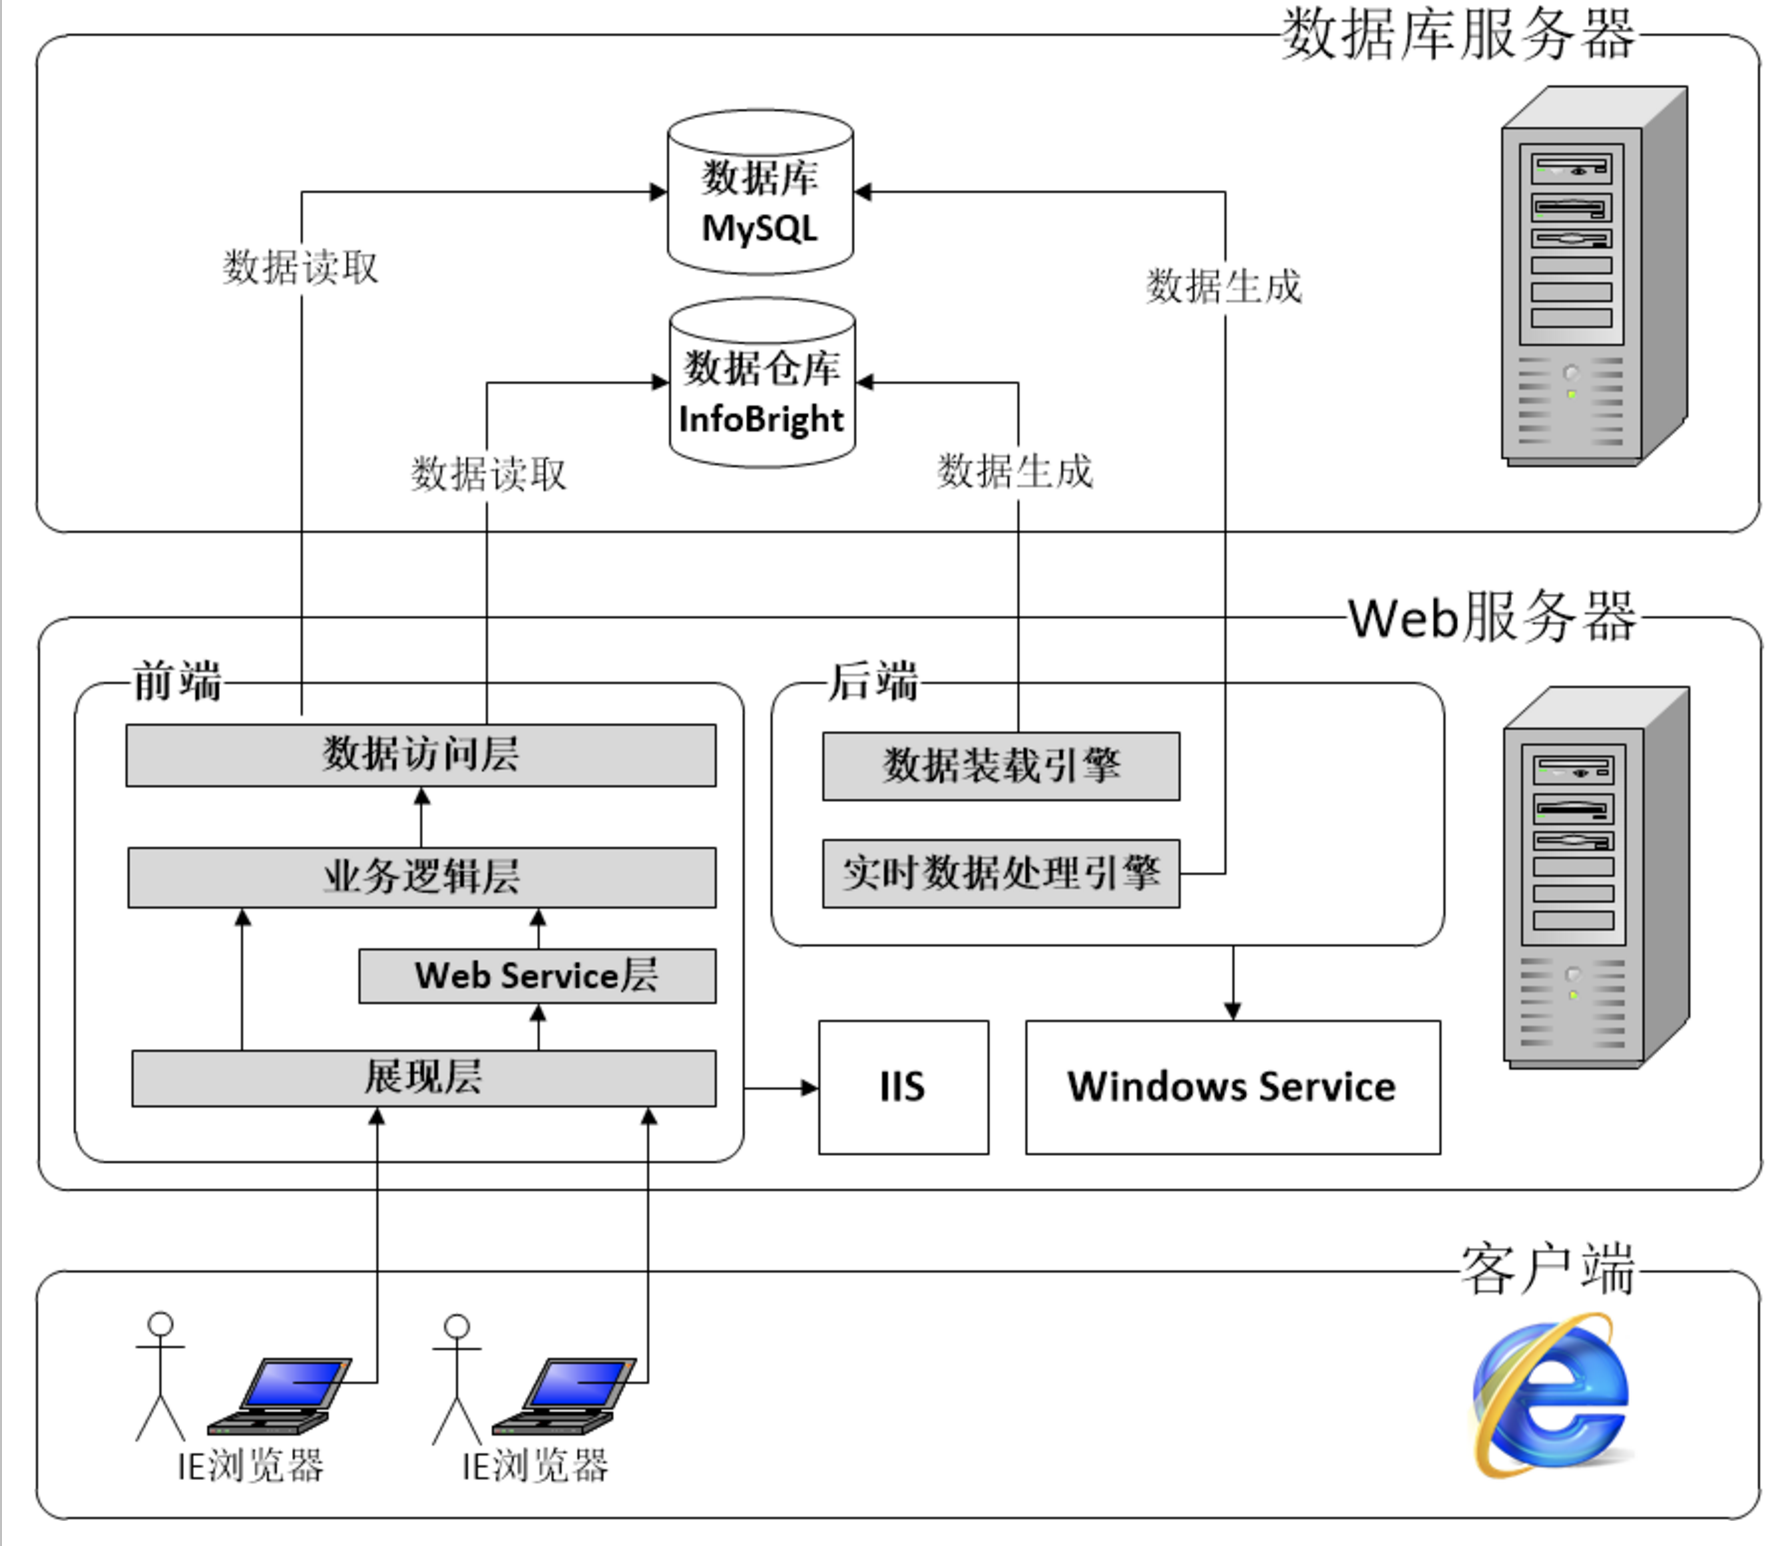
\includegraphics[width=4.4in]{picture/jiagou}
					\caption{智能高速系统架构}
					\label{fig20}
				\end{minipage}%\
		\end{figure}

		系统逻辑如图\ref{fig30}所示,首先对交通数据进行处理,剔除噪音数据,如:\ding{172}车辆在半小时时间内横跨安徽省;\ding{173}车辆丢失入口数据;\ding{174}车辆丢失出口数据等。用筛选后的数据组成车辆O-D矩阵;从数据库内抽取重大交通事故信息,结合新闻中的高速公路事故信息,计算并输入路段的损毁概率。当选取贪心算法时,系统直接根据当前输入数据,进行贪心计算,注意本系统中将关键节点维护后的损毁率下降设为0.1,具体数值可以根据实际应用调整;当选取基于社群划分的关键路段挖掘策略时,首先根据O-D流量信息计算社群分布,并给出划分结果(图\ref{fig21})、网络模块化程度,之后对每一个社群内部进行贪心求解,这个求解过程并行执行,最后结合动态规划,求得最终解集合(图\ref{fig22})。
		\begin{figure}
		\centering
				\begin{minipage}{0.8\linewidth}
					\centering
					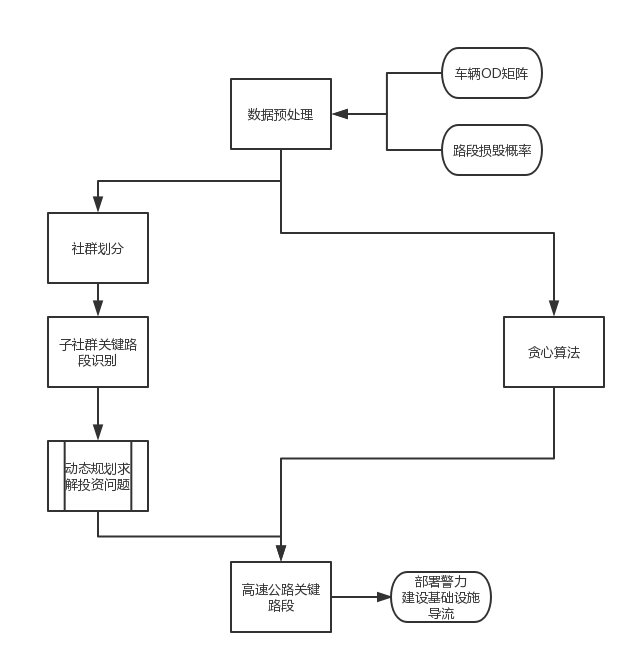
\includegraphics[width=3in]{picture/liuchengtu}
					\caption{逻辑流程图}
					\label{fig30}
				\end{minipage}%\
		\end{figure}


	\section{界面功能展示}

		系统的输入有时间,时间区间,路段损毁概率,管理者对关键路段的维护效果。

		对于静态关键路段挖掘,直接输出关键路段结果(如图\ref{fig22});对于动态关键路段挖掘,系统输出两层信息,第一层是关键路段分群效果(图\ref{fig21});第二层是关键路段选取结果(图\ref{fig22})。

				\begin{figure}[h]
				\begin{minipage}{0.5\linewidth}
					\centering
					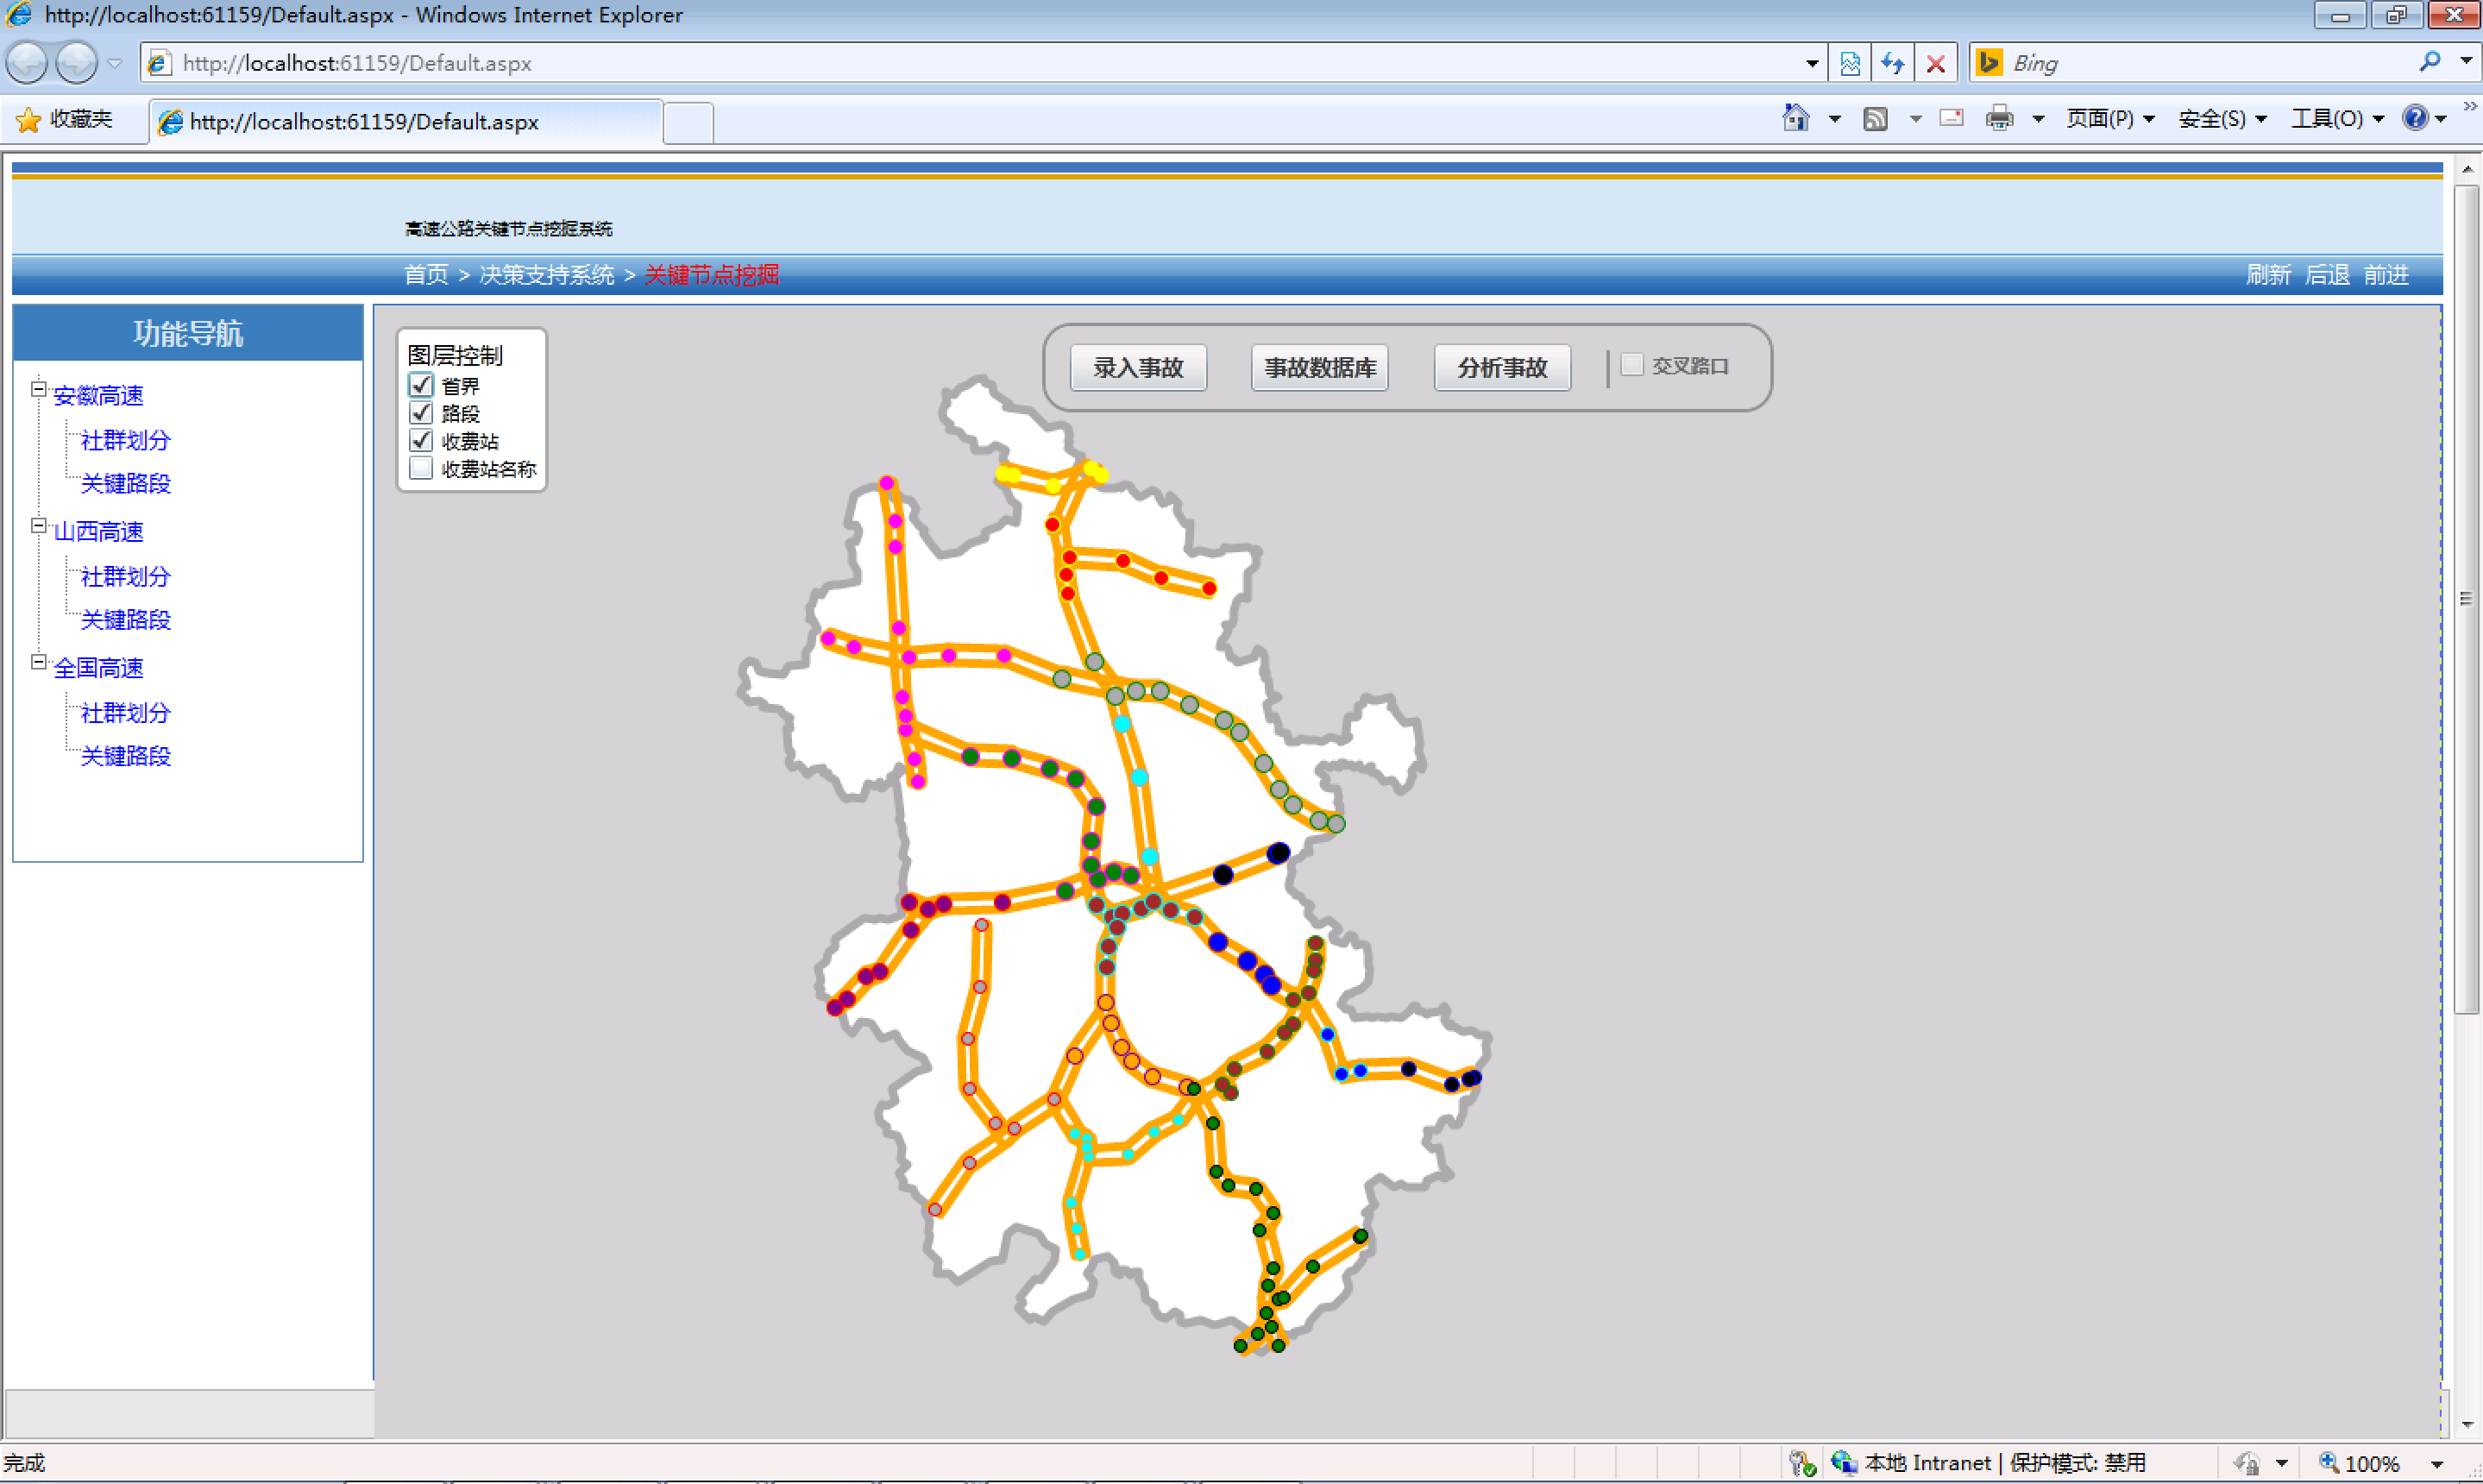
\includegraphics[width=3.0in]{picture/yuanxing1}
					\caption{系统分群结果图}
					\label{fig21}
				\end{minipage}%
				\begin{minipage}{0.5\linewidth}
					\centering
					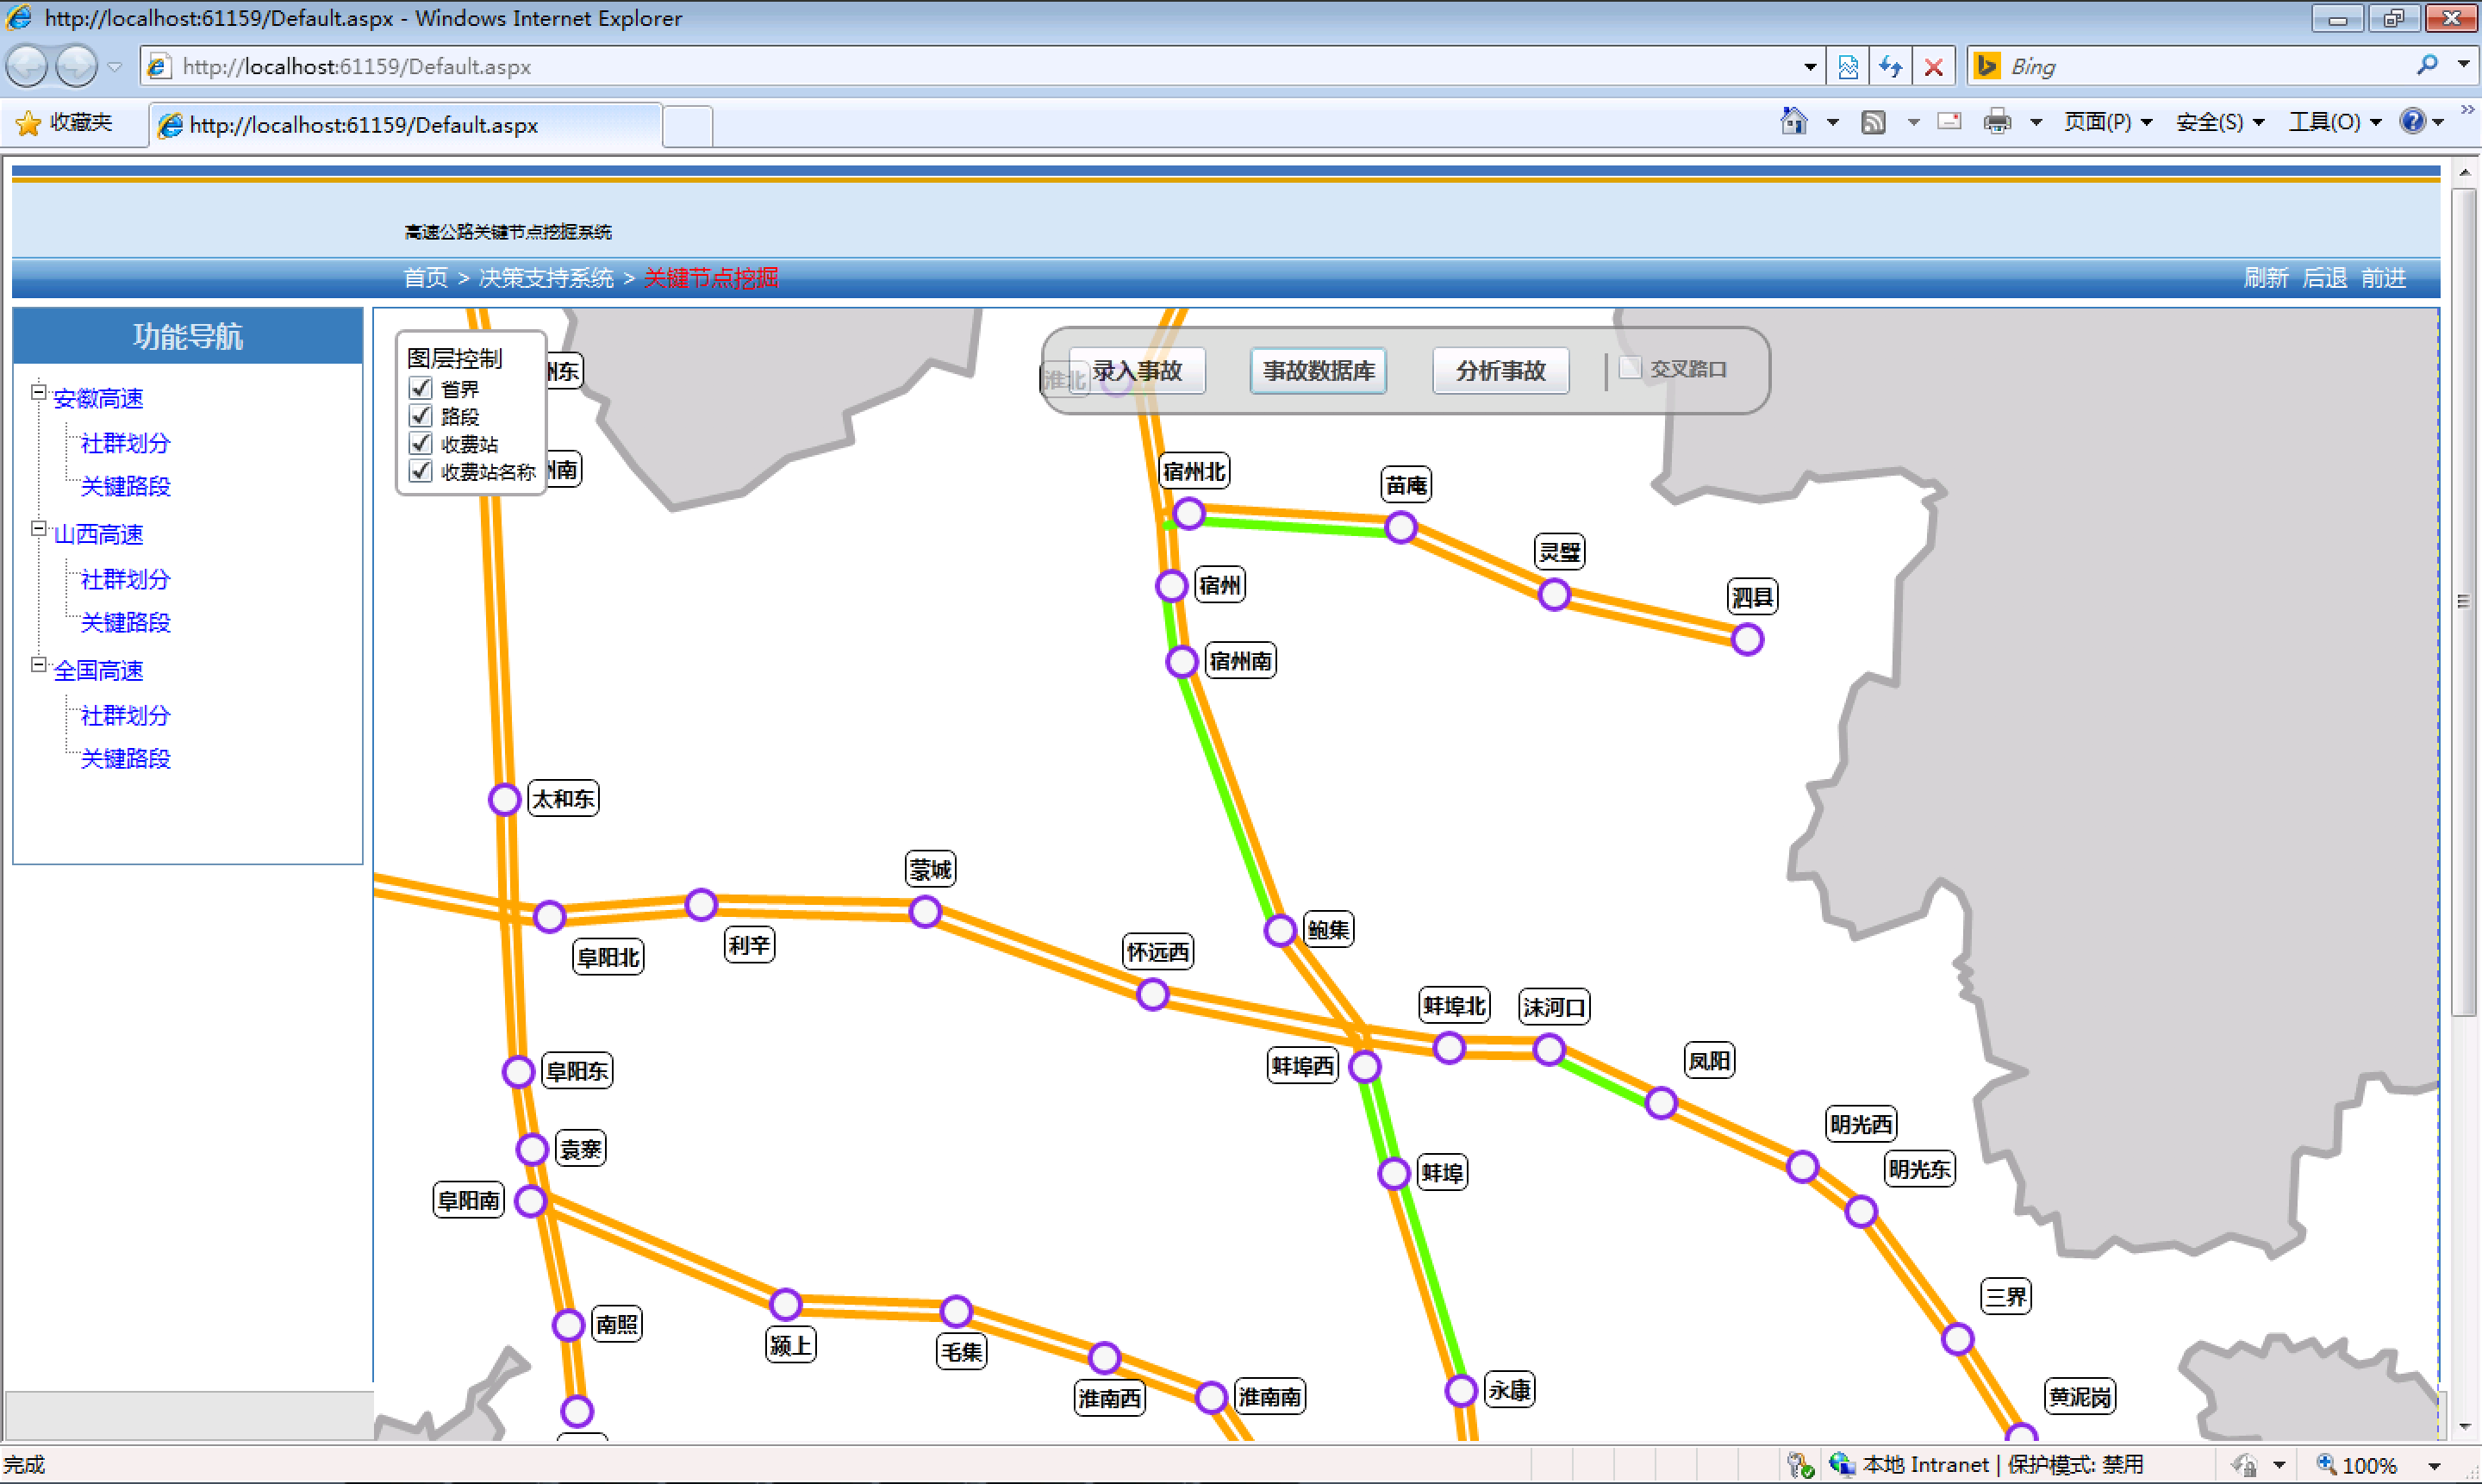
\includegraphics[width=3.0in]{picture/yuanxing2}
					\caption{系统路段选取结果图}
					\label{fig22}
				\end{minipage}
				\end{figure}



		目前系统只适用于安徽高速系统,但是可以扩展到任何具有收费站数据的中国高速公路上。

	\section{本章小结}
		本章介绍了一个面向高速公路的关键路段挖掘原型系统,给出了系统的流程图和样例图。该系统现在已经在安徽省高速公路网络上完全实现。该系统可扩展性强,所以可以很快的复用到其他省份乃至全国高速公路网络中。

	